\documentclass[conference]{IEEEtran}
\IEEEoverridecommandlockouts
\usepackage{cite}
\usepackage{amsmath,amssymb}
\usepackage{algorithm}
\usepackage{algpseudocode}
\usepackage{booktabs}
\usepackage{array}
\usepackage{tabularx}
\usepackage{graphicx}
\usepackage{tikz}
\usetikzlibrary{positioning,arrows.meta,shapes.geometric,calc}
\usepackage{pgfplots}
\usepgfplotslibrary{groupplots}
\pgfplotsset{compat=1.16}
\usepackage{url}
\def\UrlBreaks{\do\/\do-\do.}

\tikzset{
  bx/.style={draw,rounded corners=1.5pt,align=center,inner sep=2.5pt,font=\scriptsize,line width=.45pt,text width=#1},
  bx/.default=30mm,
  ar/.style={-{Latex[length=1.6mm,width=1.3mm]},line width=.5pt},
}
\pgfplotsset{
  papercurve/.style={width=\columnwidth,height=52mm,symbolic x coords={1\%,2\%,5\%,10\%},xtick=data,
    enlarge x limits=.06,ymin=0,ymax=104,ytick={0,25,50,75,100},ymajorgrids,
    grid style={line width=.2pt,draw=black!18},tick label style={font=\scriptsize},
    label style={font=\scriptsize},legend style={font=\scriptsize,draw=none,fill=none,at={(.5,1.02)},anchor=south,legend columns=2,/tikz/every even column/.append style={column sep=4pt}},
    legend cell align=left,axis lines=left,xlabel={Storage cap},ylabel={Attack signatures kept (\%)}},
}

\begin{document}

\title{Evidence-Based Retention: Reducing Packet Captures to a Byte Budget with Signature-Free Selection and Pre-Deletion Verification}

\author{\IEEEauthorblockN{Ishaan Suresh Mullya, Shriya P Reddy, Om KB}
\IEEEauthorblockA{Information Security Lab (ICT3141), B.Tech. CCE, 5th Semester\\
Faculty guide: Dr. Adesh ND}}

\maketitle

\begin{abstract}
Full packet capture is the most complete evidence a network can produce, but its storage cost forces most organizations to delete it within days. Existing reduction methods either treat all traffic alike or keep only what detection rules already recognize. We present Evidence-Based Retention (EBR), a streaming method that reduces a capture to an exact byte budget using no signatures, labels or training data. EBR scores each flow in bits of surprise under the capture's own baseline, applies a Good--Turing correction and two-level diminishing returns, and selects one fidelity level per flow as a multiple-choice knapsack. It also charges a complete flow ledger to the same budget. We then add verify before delete, a loop that scans the original and the reduced copy with an intrusion detection system and repairs losses inside the fixed budget before the original is removed. We evaluate with Suricata and 52,778 public rules as an independent judge across three sealed tests on 24.5\,GB of public captures. In a pre-registered test on scan-heavy traffic, EBR with repair preserved 99.6\% of attack signatures at a 5\% cap, against 84.9\% for IDS-triggered capture with the same rule knowledge. Only one of five pre-registered hypotheses was supported in full. We report the failures, including a scan cap that did not generalize and a login-spray blind spot in diminishing returns.
\end{abstract}

\begin{IEEEkeywords}
network forensics, packet capture, selective retention, intrusion detection, knapsack problem, pre-registration
\end{IEEEkeywords}

\section{Introduction}
Packet captures let an investigator see what was actually said on a network, long after alerts have fired. The cost is storage: a fully loaded 1\,Gbit/s link produces 10.8\,TB per day. Lossless compression does not close the gap. On our test sets gzip reached 39.9--56.5\% of the original size overall, and as much as 95.6\% on a single capture, since encrypted traffic is close to incompressible. Reaching 1--10\% of the original size requires discarding data on purpose, so the design question is \emph{which bytes an investigator would most regret losing}.

The established answers each lose something. Connection cutoffs, as in Time Machine~\cite{timemachine,timetravel}, treat every connection alike and lose late commands. Alert-triggered capture~\cite{sanspcap,suricata} keeps only what a rule already recognizes, so it cannot serve rules written after the fact. Recent traffic-aware sampling such as XNET~\cite{xnet} favors rare destinations but operates on headers. All of these methods also share a blind spot: the decision is made once, and its cost is unknown until an investigation fails.

This paper makes four contributions:
\begin{enumerate}
\item EBR, a streaming, signature-free reduction method that combines surprisal with Good--Turing correction, two-level diminishing returns, per-flow fidelity selection as a multiple-choice knapsack, and a budget-charged flow ledger.
\item Verify before delete, a repair loop that measures a reduction's losses while the original still exists and corrects them inside the same byte budget.
\item A sealed, pre-registered evaluation using an independent detector, fair comparators and paired intervals over cases.
\item Negative results that bound these claims, including an ablation showing which components matter and a blind spot in the method's most effective component.
\end{enumerate}

\section{Related Work}
\textbf{Connection-prefix retention.} Kornexl \emph{et al.}~\cite{timemachine} showed that keeping only the start of each connection preserves most value at a fraction of the volume, and Maier \emph{et al.}~\cite{timetravel} let a network IDS adjust storage classes. TrimPCAP~\cite{trimpcap} applies per-session trimming to existing files. Selective capping~\cite{capping} removes payloads that are hard to interpret later. These methods use a fixed policy per class, whereas EBR varies depth per flow by estimated value.

\textbf{Detection-driven retention.} Suricata's conditional logging~\cite{suricata} and IDS-triggered capture~\cite{sanspcap} retain traffic that matches rules. They are precise, but retention then depends on what is known at capture time.

\textbf{Traffic-aware sampling.} XNET~\cite{xnet} samples dynamically at very high rates, favoring rarely contacted destinations and DNS using header information. It runs live, which EBR does not. EBR instead reads protocol content, calibrates itself on each capture without external feeds, and optimizes against a byte budget.

\textbf{Evaluation practice.} Sommer and Paxson~\cite{outside} describe why anomaly-based intrusion detection is hard to deploy and to evaluate. Engelen \emph{et al.}~\cite{troubleshooting} document labeling and construction flaws in widely used intrusion datasets. We respond by using an independent detector, pre-registration~\cite{prereg}, and data from several sources.

\textbf{Novelty.} In a bounded literature search we found no published method with EBR's combination of parts, or one that verifies a reduction against an IDS and repairs it inside the same budget before deletion. Retention by value is not itself new, and related patents exist. Our claim concerns the combination and its evaluation.

\section{Problem Formulation}
Let a capture contain flows $F$. Each flow $f$ has packets partitioned into five fidelity tiers (Table~\ref{tab:tiers}), with byte costs $c_f(t)$ for $t\in\{0,\dots,4\}$. Choosing level $\ell_f$ retains all tiers up to $\ell_f$, and level $-1$ retains no packets. Given a budget $B$ in serialized bytes, a ledger of size $|L|$ and the PCAP framing overhead $h$, we seek
\begin{equation}
\max_{\{\ell_f\}} \sum_{f\in F} v_f(\ell_f) \quad \text{s.t.} \quad \sum_{f\in F}\sum_{t\le \ell_f} c_f(t) + |L| + h \le B.
\label{eq:mckp}
\end{equation}
This is a multiple-choice knapsack problem~\cite{mckp}. Its quality depends on the value model $v_f$, which must be computed without labels.

\begin{table}[t]
\centering
\caption{Fidelity Tiers and Value Weights}
\label{tab:tiers}
\footnotesize
\begin{tabular}{@{}llc@{}}
\toprule
Tier & Contents & Weight $w_t$\\
\midrule
0 Skeleton & SYN, FIN, RST, first and last packet & 0.20\\
1 Head & First 1\,KiB in each direction & 0.50\\
2 Deep head & First 16\,KiB in each direction & 0.15\\
3 Turn heads & First 1\,KiB of each later message turn & 0.10\\
4 Bulk & All remaining packets & 0.05\\
\bottomrule
\end{tabular}
\end{table}

\section{Evidence-Based Retention}
EBR makes two passes (Fig.~\ref{fig:pipeline}). The first streams the capture into flows, tiers and protocol fingerprints, holding no packet content. The second copies chosen records byte for byte, so the output is a standard PCAP.

\begin{figure}[t]
\centering
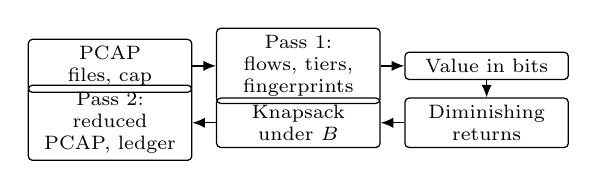
\begin{tikzpicture}[node distance=2.2mm and 3mm]
  \node[bx=19mm] (a) {PCAP files, cap};
  \node[bx=19mm,right=of a] (b) {Pass 1: flows, tiers, fingerprints};
  \node[bx=19mm,right=of b] (c) {Value in bits};
  \node[bx=19mm,below=of c] (d) {Diminishing returns};
  \node[bx=19mm,left=of d] (e) {Knapsack under $B$};
  \node[bx=19mm,left=of e] (f) {Pass 2: reduced PCAP, ledger};
  \draw[ar] (a)--(b); \draw[ar] (b)--(c); \draw[ar] (c)--(d); \draw[ar] (d)--(e); \draw[ar] (e)--(f);
\end{tikzpicture}
\caption{The EBR pipeline. No rules, labels or training data are used.}
\label{fig:pipeline}
\end{figure}

\subsection{Fidelity Tiers}
Tier positions come from TCP sequence numbers, so retransmissions fall in the tier of the data they repeat. Pure ACKs follow the data they acknowledge, which keeps retained streams usable by a reassembling IDS. Each change of speaker starts a new \emph{turn}, and Tier~3 keeps the opening of each turn, which a plain prefix cannot do. UDP tiers follow packet counts.

\subsection{Rarity}
For a trait with value $x$ seen $n_x$ times among $N$ flows, plain frequency overrates one-off values. Following Good~\cite{good}, let the novelty $g$ be the share of flows whose value occurs exactly once, and estimate
\begin{equation}
\hat{P}(x)=\max\!\left(\frac{n_x}{N},\ \frac{g}{n_x}\right),\quad s(x)=\min\bigl(16,\,-\log_2\hat{P}(x)\bigr).
\label{eq:gt}
\end{equation}
A one-off therefore scores highly only when one-offs are rare. Five traits are measured: service, flow shape, client--server pair, client fingerprint, and content skeleton. The fingerprint derives from the HTTP header layout and User-Agent, a hash of the TLS ClientHello, or the SSH banner. The skeleton replaces the words of a URL with a placeholder and keeps its punctuation, so that \texttt{/page?id=1'\%20OR\%201=1--} differs from \texttt{/page?id=7} without any rule describing SQL injection. With $e_{(i)}$ the excesses over each trait's median in descending order, rarity is
\begin{equation}
R(f)=e_{(1)}+0.25\sum_{i\ge 2} e_{(i)}.
\end{equation}

\subsection{Automation and Pivoting}
Rarity fails on floods, because a flood's traits become common. For a group of $n\ge 8$ flows sharing client, server, port and protocol,
\begin{equation}
A(f)=\log_2(n)\cdot\max\bigl(1-\sigma_{\text{size}},\ 1-\sigma_{\text{gap}},\ \phi\bigr),
\end{equation}
where $\sigma$ denotes a coefficient of variation clipped to 1 and $\phi$ is the share of failed connections. A client whose failures reach $d\ge 8$ distinct endpoints scores at least $\log_2 d$.

Let $b(f)=\max(R,A)$. A host's mass is $m(h)=\sum 2^{\min(b(f)-6,\,12)}$ over the flows it initiated with $b(f)\ge 6$, and its suspicion $H(h)$ is $\log_2(1+m(h))$ less the median across hosts, floored at zero. Each flow then receives an uplift $U(f)=0.5\max(H_{\text{client}},H_{\text{server}})$. A host that was attacked also lifts its next connections to rare peers for 30 minutes, with weight 0.25.

\subsection{Diminishing Returns}
The ten-thousandth identical failed login adds little once exemplars and an exact count exist. Within a cluster, flows are ranked, and the first 16 keep full value so that rate-based rules have an unbroken burst to fire on. The rest are visited in bit-reversed order, so any prefix covers the cluster's whole time span, and each receives a discount $r^{-p}$, where $r$ is its rank less 15. With $D_p^{C}$ this discount in cluster $C$, the multiplier is
\begin{equation}
M(f)=D_{0.5}^{\text{exact}}\cdot\min\bigl(D_{0.25}^{\text{client}},\ D_{0.25}^{\text{server}},\ D_{0.5}^{\text{silent}}\bigr).
\end{equation}
Exact repeats (same client, server, service, content and shape) fall steeply. Variations fall gently, because a new payload or endpoint is a new indicator. The client cluster omits the port, so a thousand-port scan counts as one behavior. A flow's value is then
\begin{equation}
V(f)=\bigl(1+b(f)+U(f)\bigr)\cdot M(f).
\end{equation}

\subsection{Allocation}
A level earns $v_f(\ell)=V(f)\sum_{t\le\ell} w_t$ over the tiers the flow actually occupies, so a bare SYN cannot outbid a real request by being cheap. For opaque flows, tiers above the head are worth a tenth. Algorithm~\ref{alg:alloc} reduces each flow's levels to their upper concave hull and takes segments in order of value per byte, the standard greedy solution, which is optimal for the fractional relaxation of (\ref{eq:mckp}). In the algorithm, $B$ is the budget net of the ledger and framing.

Payload-free flows are cheap enough that a scan storm can outbid content on price. On one capture they took 186\,MB of a 227\,MB packet budget. They are therefore limited to a 30\% share on the first pass, and they may use whatever content leaves unused. This second constraint makes the result a heuristic rather than the fractional optimum.

\begin{algorithm}[t]
\caption{Budgeted Level Selection}
\label{alg:alloc}
\footnotesize
\begin{algorithmic}[1]
\State $S\gets$ concave-hull segments of all flows, by value per byte
\State $\text{used}\gets 0$;\ $\text{room}\gets 0.3B$;\ $\text{deferred}\gets[\,]$
\For{each segment $(f,\ell,c)\in S$}
  \If{$f$ is blocked} \textbf{continue} \EndIf
  \If{$f$ is payload-free}
    \If{$c>\text{room}$} append to deferred; \textbf{continue} \EndIf
    \State $\text{room}\gets\text{room}-c$
  \EndIf
  \If{$\text{used}+c\le B$} $\text{used}\gets\text{used}+c$;\ $\ell_f\gets\ell$
  \Else\ block $f$ \EndIf
\EndFor
\For{each deferred segment $(f,\ell,c)$ with $\text{used}+c\le B$}
  \State $\text{used}\gets\text{used}+c$;\ $\ell_f\gets\ell$
\EndFor
\end{algorithmic}
\end{algorithm}

\subsection{Flow Ledger}
Every flow is recorded in a gzip-compressed table with its endpoints, times, packet and byte counts, application and state. When space is tight, low-value flows fold into grouped rows that keep exact totals. The ledger is limited to 10\% of the budget and is charged against $B$, so no comparator is disadvantaged.

\section{Verify Before Delete}
Retention is usually a blind bet, yet the complete capture exists until the moment it is deleted. Algorithm~\ref{alg:verify} scans both copies, finds the flows behind each lost detection, and selects again with those flows outbidding all others. The cap holds because the lowest-value evidence makes room. An alert's first repair restores its flows by five-tuple. If the alert is still lost, the next round also adds up to 64 neighboring flows between the same hosts in its time window, because rate-based rules need several flows close together.

The initial selection still uses no rules, so protection against unknown threats still rests on EBR. The IDS runs once per batch and repairs only what it can see.

\begin{algorithm}[t]
\caption{Verify Before Delete}
\label{alg:verify}
\footnotesize
\begin{algorithmic}[1]
\State $Q\gets$ IDS alerts on the full capture from admissible rules
\State $\text{forced}\gets\emptyset$;\ $\text{mask}\gets$ EBR$(B)$
\For{round $=1,2$}
  \State $\text{lost}\gets Q\setminus$ IDS alerts on the reduced copy
  \If{$\text{lost}=\emptyset$} \textbf{break} \EndIf
  \State add the flows behind lost alerts to forced
  \State for alerts repaired before and still lost, add up to 64 time-neighbors
  \State $V(f)\gets 1000\cdot\max V$ for $f\in$ forced
  \State $\text{mask}\gets$ select again under $B$
\EndFor
\State \Return mask, then delete the original
\end{algorithmic}
\end{algorithm}

\section{Evaluation Method}
\subsection{Detector and Measures}
Suricata 7.0.3 with 52,778 ET Open rules~\cite{suricata,etopen} is the judge. EBR never sees these rules during selection. We compare alerts from each reduced copy with those from the full capture. Alerts are restricted to attack categories. The primary measure is \emph{attack signature recall}, the share of distinct rules that still fire. \emph{Alert instance recall} counts distinct combinations of rule and host pair. \emph{Later-rule recall} covers rules published on or after the capture date. A case with no attack alerts on the full capture is not scored.

\subsection{Data}
Table~\ref{tab:data} lists the three sealed sets. They draw on CSE-CIC-IDS2018~\cite{cic}, WRCCDC competition captures with live human red teams~\cite{wrccdc}, CTU-Mixed captures from the group behind the CTU-13 data~\cite{ctu}, and IoT-23~\cite{iot23}. Separate development cases were used for tuning.

\begin{table}[t]
\centering
\caption{Sealed Test Sets}
\label{tab:data}
\footnotesize
\begin{tabular}{@{}lrrrl@{}}
\toprule
Test & Size & Packets & Scored & Sources\\
\midrule
First & 11.28\,GB & 35.0\,M & 6/6 & CIC (5 days), WRCCDC 2018\\
Second & 7.03\,GB & 15.1\,M & 5/6 & WRCCDC, CTU-Mixed, CIC\\
Third & 6.15\,GB & 34.0\,M & 8/9 & IoT-23, WRCCDC 2017/18\\
\bottomrule
\end{tabular}
\end{table}

\subsection{Comparators}
All methods receive the same serialized-byte budget at caps of 1, 2, 5 and 10\%. Random packet and random flow selection use three seeds. The flow cutoff, after Time Machine, is fitted to every budget, which makes it stronger than a fixed setting. Rare destinations is inspired by XNET but is not a reproduction, since it is offline and uses no popularity feeds. IDS-triggered + fill keeps alerted flows and spends what remains on a fitted cutoff. It receives real alerts from rules older than each capture, an advantage EBR's first selection never has. Repair in the third test used the same restricted rules.

\subsection{Sealing and Pre-Registration}
Before each test, code, settings and scoring were hashed with SHA-256 and recorded, and only then were the captures opened. For the third test, the plan itself was included among 22 hashed files. It fixed the primary measure, the pass rule and these hypotheses:
\begin{itemize}
\item H1: on scan-heavy cases, EBR with the scan cap beats the first version at 5\% and 10\%.
\item H2: repair beats EBR alone at every cap.
\item H3: repair beats IDS-triggered + fill at every cap.
\item H4: repair costs later-rule recall at most 5 points on average at any cap.
\item H5: a hidden-family estimate of unknown-threat recall beats guessing the mean, given at least 10 usable pairs.
\end{itemize}
A blind screen using packet headers alone, run before any detection, marked 7 of the 9 captures as scan-heavy. The first frozen run stopped on a PCAPNG file before any scoring. The file was converted, Scapy confirmed 18,890,171 packets with zero mismatches, and no frozen file changed.

\subsection{Statistics}
A hypothesis counts as supported at a cap only if the mean paired difference favors it and the 95\% bootstrap interval~\cite{bootstrap}, from 10,000 resamples of cases, excludes zero.

\section{Results}
\subsection{Across the Three Tests}
Table~\ref{tab:all} gives signature recall at a 5\% cap. In the first test, EBR beat the tuned cutoff and rare destinations with intervals excluding zero at every cap, and it could not be separated from IDS-triggered capture. It preserved all 8 labeled attacks that the detector finds on complete captures at 5\% and 10\%. Its ledger gave the exact attacker flow count in all five labeled cases at 5\%. The weak spot was a human red-team capture (60.7\% against 78.6\%), where diagnosis found payload-free flows taking 82\% of the budget, which led to the scan cap.

In the second test, EBR led every comparator on signature recall at every cap, clearing the interval against IDS-triggered capture at 5\% and 10\% (+8.5 and +6.5 points). However, the scan cap never engaged, because payload-free flows would have taken at most 3.4\% of the budget. The third test was designed to fix this gap.

\begin{table}[t]
\centering
\caption{Attack Signature Recall (\%) at a 5\% Cap}
\label{tab:all}
\footnotesize
\begin{tabular}{@{}lrrrrr@{}}
\toprule
Test & EBR & Repair & IDS+fill & Cutoff & Rare\\
\midrule
First & 91.7 & -- & 86.5 & 62.8 & 69.2\\
Second & 94.4 & -- & 85.9 & 77.5 & 79.9\\
Third & 84.7 & \textbf{99.6} & 84.9 & 34.4 & 14.1\\
\bottomrule
\end{tabular}
\end{table}

\subsection{Third Sealed Test}
Fig.~\ref{fig:third} and Table~\ref{tab:third} show the results on scan-heavy data. Table~\ref{tab:hyp} gives the verdicts: one hypothesis was supported in full. Repair beat EBR alone at every cap (Fig.~\ref{fig:forest}). It beat IDS-triggered capture clearly at 2, 5 and 10\%, but not at 1\%, so H3 fails under the pre-registered rule. EBR alone fell behind IDS-triggered capture at 1\% and 2\%, drew level at 5\% and led at 10\%, so its earlier lead does not hold on all traffic.

\begin{figure}[t]
\centering
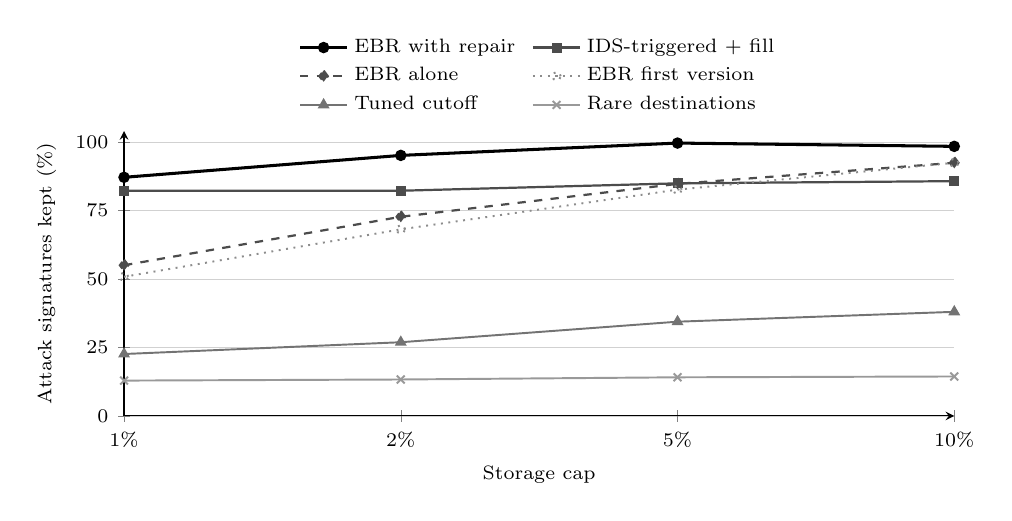
\begin{tikzpicture}
\begin{axis}[papercurve]
\addplot[black,line width=1.1pt,mark=*,mark size=1.5pt] coordinates {(1\%,87.1)(2\%,95.1)(5\%,99.6)(10\%,98.4)};
\addplot[black!70,line width=.8pt,mark=square*,mark size=1.4pt] coordinates {(1\%,82.2)(2\%,82.2)(5\%,84.9)(10\%,85.7)};
\addplot[black!70,line width=.8pt,dashed,mark=diamond*,mark size=2pt] coordinates {(1\%,55.0)(2\%,72.7)(5\%,84.7)(10\%,92.4)};
\addplot[black!45,line width=.7pt,dotted,mark=o,mark size=1.5pt] coordinates {(1\%,50.8)(2\%,68.1)(5\%,82.6)(10\%,92.4)};
\addplot[black!55,line width=.7pt,mark=triangle*,mark size=1.8pt] coordinates {(1\%,22.6)(2\%,26.9)(5\%,34.4)(10\%,38.0)};
\addplot[black!40,line width=.7pt,mark=x,mark size=2pt] coordinates {(1\%,12.9)(2\%,13.3)(5\%,14.1)(10\%,14.4)};
\legend{EBR with repair,IDS-triggered + fill,EBR alone,EBR first version,Tuned cutoff,Rare destinations}
\end{axis}
\end{tikzpicture}
\caption{Third sealed test: attack signature recall, mean over 8 scored cases.}
\label{fig:third}
\end{figure}

\begin{table}[t]
\centering
\caption{Third Test: Recall (\%) by Cap}
\label{tab:third}
\footnotesize
\begin{tabular}{@{}lrrrr@{}}
\toprule
Attack signatures & 1\% & 2\% & 5\% & 10\%\\
\midrule
EBR with repair & \textbf{87.1} & \textbf{95.1} & \textbf{99.6} & \textbf{98.4}\\
EBR alone & 55.0 & 72.7 & 84.7 & 92.4\\
EBR first version & 50.8 & 68.1 & 82.6 & 92.4\\
IDS-triggered + fill & 82.2 & 82.2 & 84.9 & 85.7\\
Tuned flow cutoff & 22.6 & 26.9 & 34.4 & 38.0\\
Rare destinations & 12.9 & 13.3 & 14.1 & 14.4\\
\midrule
Alert instances & 1\% & 2\% & 5\% & 10\%\\
\midrule
EBR with repair & \textbf{79.3} & \textbf{85.3} & \textbf{92.2} & \textbf{94.2}\\
EBR alone & 40.3 & 49.7 & 74.2 & 85.3\\
IDS-triggered + fill & 73.1 & 73.3 & 82.0 & 82.2\\
\bottomrule
\end{tabular}
\end{table}

\begin{table}[t]
\centering
\caption{Pre-Registered Verdicts}
\label{tab:hyp}
\footnotesize
\begin{tabular}{@{}l l p{51mm}@{}}
\toprule
& Verdict & Difference in points [95\% interval]\\
\midrule
H1 & Not supported & 5\%: +2.8 [0.0, +8.3]; 10\%: 0.0 [0.0, 0.0]\\
H2 & Supported & 1\%: +32.1 [+10.6, +54.5]; 2\%: +22.4 [+3.4, +43.3]; 5\%: +14.9 [+3.4, +28.8]; 10\%: +7.6 [+0.4, +19.7]\\
H3 & Not supported & 1\%: +4.8 [$-$14.4, +21.4]; 2\%: +12.9 [+3.6, +23.4]; 5\%: +14.7 [+4.2, +25.7]; 10\%: +12.7 [+3.3, +22.1]\\
H4 & Not supported & 1\%: $-$1.7; 2\%: $-$7.5 (four cases); 5\%: 0.0; 10\%: 0.0\\
H5 & Not scoreable & 8 of 10 pairs. Error 24.5 vs.\ 14.6 for guessing\\
\bottomrule
\end{tabular}
\end{table}

\begin{figure}[t]
\centering
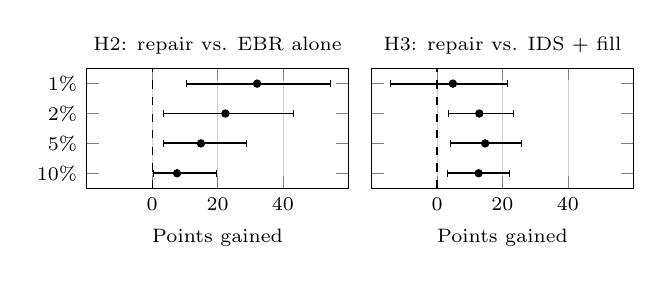
\begin{tikzpicture}
\begin{groupplot}[group style={group size=2 by 1,horizontal sep=3mm},width=49mm,height=31mm,
  ytick={1,2,3,4},yticklabels={10\%,5\%,2\%,1\%},ymin=.5,ymax=4.5,xmin=-20,xmax=60,xtick={0,20,40},
  tick label style={font=\scriptsize},label style={font=\scriptsize},title style={font=\scriptsize,yshift=-1.5mm},
  xmajorgrids,grid style={line width=.2pt,draw=black!18},xlabel={Points gained}]
\nextgroupplot[title={H2: repair vs. EBR alone}]
\addplot[only marks,mark=*,mark size=1.3pt,black,error bars/.cd,x dir=both,x explicit,error bar style={line width=.7pt}] coordinates {
 (32.1,4) += (22.4,0) -= (21.5,0)
 (22.4,3) += (20.9,0) -= (19.0,0)
 (14.9,2) += (13.9,0) -= (11.5,0)
 (7.6,1) += (12.1,0) -= (7.2,0)};
\draw[black,dashed,line width=.5pt] (axis cs:0,.5) -- (axis cs:0,4.5);
\nextgroupplot[title={H3: repair vs. IDS + fill},yticklabels={}]
\addplot[only marks,mark=*,mark size=1.3pt,black,error bars/.cd,x dir=both,x explicit,error bar style={line width=.7pt}] coordinates {
 (4.8,4) += (16.6,0) -= (19.2,0)
 (12.9,3) += (10.5,0) -= (9.3,0)
 (14.7,2) += (11.0,0) -= (10.5,0)
 (12.7,1) += (9.4,0) -= (9.4,0)};
\draw[black,dashed,line width=.5pt] (axis cs:0,.5) -- (axis cs:0,4.5);
\end{groupplot}
\end{tikzpicture}
\caption{Paired differences with 95\% bootstrap intervals. The dashed line marks zero.}
\label{fig:forest}
\end{figure}

\textbf{Costs of repair.} Repaired flows used 15.6, 13.1, 5.0 and 1.4\% of the budget at the four caps. Repair made 3 of 64 case comparisons worse, and 249 of 2,041 usable alerts stayed lost at 5\%, mostly rate-based scan rules. Scanning the original took about 62\,s per GB in our lab, in addition to about 20\,s per GB for profiling and scoring.

\textbf{Measurement noise.} Scanning identical selections twice changed 12 of 32 comparisons, by 0.4 points of instance recall on average and 6.1 at most. Signature recall moved by 0.4 points on average and 12.5 at most, on a case with only 8 signatures. Single-threaded scanning did not remove this, so gaps of a point or two are not meaningful.

\subsection{Ablation}
Table~\ref{tab:abl} removes one component at a time on the first test's data. Diminishing returns accounts for most of the benefit, cutting recall at 1\% from 87.7\% to 51.5\% when removed. Removing pivoting or turn heads changed nothing measurable. Removing the ledger raised labeled attacks caught at 1\% from 5 to 7, which is the price of exact flow accounting.

\begin{table}[t]
\centering
\caption{Ablation: Signature Recall (\%), First Test}
\label{tab:abl}
\footnotesize
\begin{tabular}{@{}lrrrr@{}}
\toprule
Variant & 1\% & 2\% & 5\% & 10\%\\
\midrule
Full EBR & 87.7 & 90.5 & 91.7 & 91.1\\
No diminishing returns & 51.5 & 67.3 & 77.8 & 77.8\\
Tiers and knapsack only & 51.1 & 63.4 & 75.5 & 76.5\\
No rarity & 83.8 & 88.6 & 91.1 & 92.3\\
No automation & 87.1 & 89.9 & 90.5 & 91.7\\
No pivoting & 87.7 & 90.5 & 91.7 & 91.1\\
No turn heads & 87.7 & 90.5 & 91.7 & 91.1\\
No ledger & 87.7 & 90.5 & 91.7 & 92.3\\
\bottomrule
\end{tabular}
\end{table}

\section{Discussion}
\textbf{Why the scan cap failed.} On IoT captures a botnet host produces millions of scan flows but few with content, and that content usually fits anyway. The cap helped 3 of 8 cases and did not lower signature recall in any. It is a safeguard against a rare failure, not a general gain.

\textbf{Login sprays.} On the Hide and Seek capture, EBR alone lost 110 of 158 attack alert instances at a 10\% cap, mostly Telnet logins with default passwords, the technique Mirai made well known~\cite{mirai}. Attempts share size and shape and differ only in the password, so diminishing returns treats them as repeats. This is a real blind spot in the component that does the most work. Repair corrects it when a rule exists.

\textbf{Later-published rules.} In the first test, rules newer than the capture did not favor EBR as we had expected (85.0\% against 92.9\% at 5\%), because new rules mostly fired on flows that older rules had flagged. In the third test H4 narrowly failed on only four cases. The blind-spot estimate looked promising on unsealed data, then did worse than guessing on the few usable pairs, so we regard it as unproven.

\textbf{Threats to validity.} Each test has few independent cases, so intervals are wide. Many cases come from one generated dataset, which has known limitations~\cite{troubleshooting}. IoT-23 captures are the first 300\,MB of longer recordings and are dominated by one infected host. The WRCCDC 2018 slices share an event with a development capture, at different hours. All three test sets have now been seen, so they cannot serve as sealed data again. We measured what a rule-based detector can find, not what a human analyst can reconstruct. Reduced captures can also raise a few alerts absent from the full capture, and every method showed this.

\textbf{Limitations.} EBR runs offline in two passes and is not a detector, since its suspect list is a triage aid. Discarded data cannot be recovered. Rate-based rules are hard to repair. At about 82\,s per GB, a single machine like ours could sustain roughly 100\,Mbit/s, so faster links would need parallel batches. Pre-deletion scanning requires an IDS and compute. SHA-256 freezes show that files are unchanged, which is not the same as a chain of custody~\cite{nist86}.

\section{Conclusion}
EBR shows that a signature-free, value-driven method can reach 1--10\% of the original size while preserving most detections, and that behavior-aware diminishing returns is what makes this work under tight caps. The stronger result is verify before delete. Measuring losses while the original exists and repairing them inside the same budget kept 99.6\% of attack signatures at a 5\% cap in a pre-registered sealed test. Most of our pre-registered hypotheses did not pass in full, and we report that plainly.

Future work should make content comparison sensitive to credentials so that sprays stop resembling repeats, retest the blind-spot estimate on captures with more later-published rules, evaluate on operational networks, build a streaming version, and measure analyst performance on reduced evidence.

\section*{Data and Code Availability}
All captures are from public sources. The implementation, pre-registered plan, SHA-256 freeze records and per-case results are kept in the project archive and are available from the authors.

\section*{Acknowledgment}
The authors thank Dr.\ Adesh ND for guidance during this work. Under IEEE's policy on AI-generated content, the authors disclose that Claude (Anthropic), running in Claude Code, was used for the EBR implementation, the evaluation harness, all figures, and the drafting of every section of this paper, at a substantial level. An earlier version of the project was produced with ChatGPT (OpenAI). The experimental results come from executed code and saved outputs, and the authors are responsible for the content.

\IEEEtriggeratref{15}
\begin{thebibliography}{99}
\bibitem{timemachine} S.~Kornexl, V.~Paxson, H.~Dreger, A.~Feldmann, and R.~Sommer, ``Building a time machine for efficient recording and retrieval of high-volume network traffic,'' in \emph{Proc. ACM SIGCOMM Internet Meas. Conf.}, 2005, pp.~267--272.
\bibitem{timetravel} G.~Maier, R.~Sommer, H.~Dreger, A.~Feldmann, V.~Paxson, and F.~Schneider, ``Enriching network security analysis with time travel,'' in \emph{Proc. ACM SIGCOMM}, 2008, pp.~183--194.
\bibitem{sanspcap} Z.~Gaster, ``Rethinking full packet capture: Evaluating IDS-triggered PCAP,'' SANS Institute, White Paper, Sep. 2026.
\bibitem{suricata} Open Information Security Foundation, ``Suricata user guide.'' Accessed: Oct. 2026. [Online]. Available: \url{https://docs.suricata.io}
\bibitem{xnet} T.~Papastergiou \emph{et~al.}, ``XNET: Intelligent dynamic sampling for high-speed network security monitoring,'' arXiv:2608.18349, Aug. 2026.
\bibitem{trimpcap} E.~Hjelmvik, ``Don't delete PCAP files -- trim them!'' Netresec Blog, Dec. 2017.
\bibitem{capping} V.~Uceda, M.~Rodr\'iguez, J.~Ramos, J.~L.~Garc\'ia-Dorado, and J.~Aracil, ``Selective capping of packet payloads for network analysis and management,'' in \emph{Proc. Traffic Monit. Anal. (TMA)}, ser. LNCS, vol. 9053, 2015.
\bibitem{outside} R.~Sommer and V.~Paxson, ``Outside the closed world: On using machine learning for network intrusion detection,'' in \emph{Proc. IEEE Symp. Secur. Privacy}, 2010, pp.~305--316.
\bibitem{troubleshooting} G.~Engelen, V.~Rimmer, and W.~Joosen, ``Troubleshooting an intrusion detection dataset: The CICIDS2017 case study,'' in \emph{Proc. IEEE Secur. Privacy Workshops}, 2021, pp.~7--12.
\bibitem{prereg} B.~A.~Nosek, C.~R.~Ebersole, A.~C.~DeHaven, and D.~T.~Mellor, ``The preregistration revolution,'' \emph{Proc. Nat. Acad. Sci. USA}, vol.~115, no.~11, pp.~2600--2606, 2018.
\bibitem{mckp} P.~Sinha and A.~A.~Zoltners, ``The multiple-choice knapsack problem,'' \emph{Oper. Res.}, vol.~27, no.~3, pp.~503--515, 1979.
\bibitem{good} I.~J.~Good, ``The population frequencies of species and the estimation of population parameters,'' \emph{Biometrika}, vol.~40, nos.~3--4, pp.~237--264, 1953.
\bibitem{etopen} Proofpoint, ``Emerging Threats Open ruleset.'' Accessed: Oct. 2026. [Online]. Available: \url{https://rules.emergingthreats.net}
\bibitem{cic} I.~Sharafaldin, A.~H.~Lashkari, and A.~A.~Ghorbani, ``Toward generating a new intrusion detection dataset and intrusion traffic characterization,'' in \emph{Proc. 4th Int. Conf. Inf. Syst. Secur. Privacy}, 2018, pp.~108--116.
\bibitem{wrccdc} Western Regional Collegiate Cyber Defense Competition, ``Public archive.'' Accessed: Oct. 2026. [Online]. Available: \url{https://archive.wrccdc.org}
\bibitem{ctu} S.~Garc\'ia, M.~Grill, J.~Stiborek, and A.~Zunino, ``An empirical comparison of botnet detection methods,'' \emph{Comput. Secur.}, vol.~45, pp.~100--123, 2014.
\bibitem{iot23} S.~Garcia, A.~Parmisano, and M.~J.~Erquiaga, ``IoT-23: A labeled dataset with malicious and benign IoT network traffic,'' Zenodo, 2020. [Online]. Available: \url{https://zenodo.org/record/4743745}
\bibitem{bootstrap} B.~Efron and R.~J.~Tibshirani, \emph{An Introduction to the Bootstrap}. New York, NY, USA: Chapman \& Hall, 1993.
\bibitem{mirai} M.~Antonakakis \emph{et~al.}, ``Understanding the Mirai botnet,'' in \emph{Proc. 26th USENIX Secur. Symp.}, 2017, pp.~1093--1110.
\bibitem{nist86} K.~Kent, S.~Chevalier, T.~Grance, and H.~Dang, ``Guide to integrating forensic techniques into incident response,'' Nat. Inst. Standards Technol., Gaithersburg, MD, USA, Special Publication 800-86, Aug. 2006.
\end{thebibliography}

\end{document}
